\section{Learning to describe new objects from corpora}
\label{sec:learning}

In the previous section we presented an algorithm that assumes that each relation R 
used in a referring expressions has a known probability of use R.\puse. In this section, 
we describe how to calculate these probabilities from corpora.  
The general set up is the following: we assume available a corpus of REs associated 
to different scenes that are typical of the domain in which the GRE algorithm will have to operate.   
We show first how to calculate R.\puse\ values for those scenes for which a corpus of REs is available.  
We then show how to generalize these values to 
other scenes in the domain, using a machine learning algorithm. \textit{First we} will exemplify the methodology using 
the GRE3D7 corpus which we introduce in the Section ~\ref{sec:learningGRE} and then we will show how to do the same with the TUNA-corpus 
that we describe in Section~\ref{sec:learningTUNA}.

\subsection{\textit{The GRE3D7:} A corpus of referring expressions}
\label{sec:learningGRE}

The GRE3D7 corpus of~\shortcite{viet:gene11} consists of 4480 referring expressions. 
It is the largest corpus of distinguishing descriptions developed to date. 
The REs in the corpus describe objects in 32 3D scenes. Each scene contains a small number of simple objects 
(cubes and balls), and the individual descriptions were elicited in the absence of a preceding discourse. 
The stimulus scenes are designed in a way that encourage the use of relations between objects, but do not require them 
(i.e., a purely propositional RE for the target always exists). For a detailed description of the collection procedure 
see~\cite[Chapter 5]{viet:gene11}. A sample scene used in the corpus collection is shown in Figure~\ref{GRE3D7-stimulus} 
(the target object is marked with an arrow). Table~\ref{corpus-distribution} shows the REs that appear in the corpus for 
Figure~\ref{GRE3D7-stimulus} together with their total number of occurrences and the percentage these totals represent.  

\begin{table}[h!]
\begin{center}
\begin{tabular}{|l|c|c|}
\hline
Referring expressions & Occurrences & Percentage \\
\hline
green ball & 91 & 65.00\% \\
small green ball & 23 & 16.43\% \\
small green ball on top of large blue cube & 8 & 5.71\% \\
green ball on top of blue cube & 5 & 3.57\% \\
green ball on top of large blue cube & 5 & 3.57\% \\
small green ball on top of blue cube & 2 & 1.43\% \\
ball on top of cube & 1 & 0.71\% \\
small green ball on top of large blue cube to the left & 1 & 0.71\% \\
small ball on top large cube & 1 & 0.71\% \\
green ball on top & 1 & 0.71\% \\
small ball on top of small cube & 1 & 0.71\% \\
green ball on top of cube & 1 & 0.71\% \\
\hline
\end{tabular}
\caption{Referring expressions produced by the subjects for Figure~\ref{GRE3D7-stimulus}\label{corpus-distribution}}
\end{center}
\end{table}

The REs in the corpus were produced by 294 participants, each participant producing 16 referring expressions corresponding to 16 
different scenes. In this way, 140 descriptions for each of the 32 scenes were obtained, resulting in a corpus of 4480 REs in total. 

\todo{Add closing paragraph}

\subsection{The TUNA-corpus: A corpus of referring expressions}
\label{sec:learningTUNA}

The TUNA (Towards a UNified Algorithm for the generation of referring expressions) Corpus (Gatt et al., 2007), is a set of human-produced referring expressions (REs) for entities in visual domains of
pictures of furniture or people. The corpus was
collected during an online elicitation experiment in
which 50 native or fluent speakers of English typed descriptions for 38 different figures of a target referent
in a domain in which there were also 6 other entities (‘distractors’). 
Each scene contains the target and distractors with theirs properties, the RE given for a human, and the semantic annotation of this.   
They show a figure that contains the pictures of furnitures or people in a grid 5x3 like in the following figure, whit the target object maket with a red rectangle.

\begin{figure}[ht] 
\centering
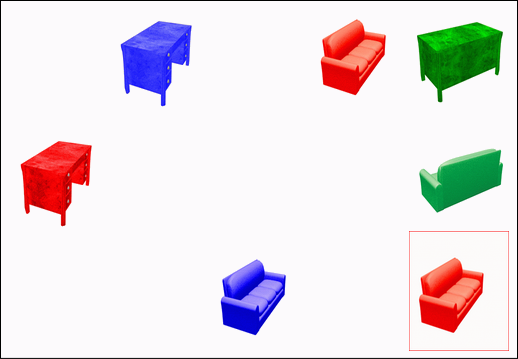
\includegraphics[width=.6 \textwidth]{images/imagen.png}
\caption{TUNA: picture of furniture}
\label{picture_furniture}
\end{figure}

The TUNA Corpus was annotated with the main objective to evaluate the output of algorithms for the Generation of Referring Expressions (GRE) with Natural Language Generation, with particular regard for the semantic content of the expressions.

A characteristic of this corpus is that have 1 RE for each scene and it contains about 2000 descriptions.


\subsection{Calculating \puse\ when a corpus for the scene is available}

Suppose we want to automatically generate REs for target $t$ in a given scene, and that we do have available a corpus $C$ 
of REs for $t$ in that scene (this is exactly the kind of information we find in the GRE3D7 corpus \textit{and in the TUNA-corpus}).  
We use the REs in $C$ to define the relational model 
used by the algorithm.  Then we estimate the value of \puse\ for each of the relations in the model as the percentage of REs 
in which the relation appears.  I.e., 
\begin{equation}\label{eq1}
R.\puse = \frac{\# \mbox{ of REs in $C$ in which R appears}}{\# \mbox{ of REs in $C$}}.
\end{equation}

\noindent
This estimation is overly simplified and, for example, it does not differentiate between the properties of a target and the 
properties of a landmark object used in a relational RE to complete the description of the target.  But it is extremely easy 
to compute, and we will see in Section~\ref{sec:evaluation} that it already produces natural REs that match those found in the corpus. 

To clarify the computation of R.\puse\ and the model $\gM$ associated to each scene we list the required steps in detail, 
and discuss how we carried them out in the GRE3D7 corpus:

\vspace*{-.4cm}
\begin{enumerate}
\item Tokenize the referring expressions and call the set of tokens $T$. In particular, multi-word expressions like ``on top of'' 
should be matched to a single token like \emph{ontop}.\\[-1.9em]

\item Remove hyperonyms from $T$. E.g., if both \emph{cube} and \emph{thing} appear in $T$, delete \emph{thing}.\\[-2em]

\item If the set of tokens obtained in the previous steps contains synonyms normalize them to a representative in the synonym class, 
and call the resulting set $\REL$; it will be the signature of the model $\gM$ used by the algorithm. E.g., the tokens \emph{little} 
and \emph{small} are both represented by the token \emph{small}.\\[-1.9em]

\item For each scene, define $\gM$ such that the interpretation $\interp{\cdot}$ ensures that all the REs in the corpus are REs in the model.
 E.g., the $\el$ formulas corresponding to the REs in Table~\ref{corpus-distribution} should all denote the target in the model $\gM$ 
depicted in 
Figure~\ref{GRE3D7-stimulus-graph}.\\[-1.9em]

\item For each R $\in \REL$ compute R.\puse\ using~(\ref{eq1}).\\[-1.9em]

\end{enumerate}

Steps 1-5 above are easy to carry out (actually, the tokenization and normalization steps were already done in the GRE3D7 corpus). 
Starting from the scene in Figure~\ref{GRE3D7-stimulus} and the corresponding corpus shown in Table~\ref{corpus-distribution}, 
the resulting signature and their associated \puse\ are listed in the first three columns of Table~\ref{probability-of-use}. 

Notice that the values R.\puse\ obtained in this way should be interpreted as the probability of using R to describe the target in model 
$\gM$, and we could argue that they are correlated to the \emph{saliency} of R in the model.  
For that reason, for example, the value of \emph{ball}.\puse\ is 1, while the value of \emph{cube}.\puse\ is 0.178.  
These probabilities will not be useful to describe different targets in different scenes.  We will see how we can use them to obtain
 values for new targets and scenes using a machine learning approach in the next section.  Not surprisingly, using these values for 
R.\puse\ the REs generated most often by the algorithm can be found in the corpus.  More interestingly, as we discuss in 
Section~\ref{sec:evaluation} the algorithm generates REs with a distribution that matches the one found in the corpus and, 
as Table~\ref{results-algo-fig3} shows, even the generated REs not found in the corpus are natural.    


\subsection{Calculating \puse\ for scenes without corpora for the target} \label{subsec:learning}

If there is no corpora that describes the target we can estimate the \puse from corpora on a different scenes in the same domain. 

We use simple features to obtain the function, all the features can be extracted automatically from the relational model 
and are listed 
in Table~\ref{features}.  

\begin{small}
\begin{table}[h!]
\begin{center}
\begin{tabular}{|l|p{10cm}|}
\hline
target & whether the target element has the property \\
\#rel-prop & number of properties and relations that the target has\\
\#rel & number of the relations that the target has \\
landmark & whether a landmark of the target has the property, an object is a landmark if there is a direct relation in the model 
between them \\
discrimination & 1 over the number of objects in the model that have the property \\
\hline
\end{tabular}
\caption{Features used for learning the \puse ~for each token in the signature of the scenes \textit{(GRE3D7 and TUNA-corpus)} \label{features}}
\end{center}
\end{table}
\end{small}

Our feature set is intentionally simplistic in order for it to be domain independent. As a result there are some complex relations 
between characteristics of the scenes that it is not able to capture. The most important characteristic of the GRE3D7 domain is that we are not able 
to learn, and has an impact in our performance, the properties of type size (namely, small and large) are used much more 
when the target cannot be uniquely identified with taxonomical (ball and cube) and absolute (green and blue) properties only. 
In other words, in the GRE3D7 corpus the size is used more often (90.2\%) of the time when the resulting RE is not overspecified 
than when it is (34\%). It may not be possible to learn this characteristic from the GRE3D7 data since even with the domain dependent 
features defined in~\cite[Chapter 6]{viet:gene11}, it could not be learned by decision trees. As a result we can see in 
Table~\ref{probability-of-use} that for Fig 13 the value estimated for ``large'' are not close to the value calculated from corpora. 
\textit{In the case of the TUNA-corpus we show that we couldn't learn the dependency of dimension-x and dimension-y, it mean, when a person adds 
dimension-x is highly probably that he includes dimension-y in his referring expression.}
\begin{table}[h!]
\begin{center}
\begin{tabular}{|l|c|c|c|c|}
\hline
Token & Model Fig 3 \puse & Learned Fig 3\puse & Model Fig 13 \puse & Learned Fig 13 \puse \\
\hline
ball & 1.0 & 1.0 & 1.0 & 1.0 \\
cube & 1.0 & 1.0 & 1.0 & 1.0 \\
green & 0.978 & 0.993 & 1.0 & 0.9875 \\
small & 0.257 & 0.346 & 0.0428 & 0.1993 \\
on-top & 0.178 & 0.179 & 0 & 0\\ 
blue & 0.15 & 0.124 & 0.064 & 0.1353 \\
large & 0.107 & 0.03 & 0.307 & 0.7378 \\
left & 0.007 & 0.002 & 0 & 0.0024 \\
top & 0.007 & 0 & 0 & 0 \\
right & 0 & 0.001 & 0.064 & 0.0005 \\
left-of & 0 & 0 & 0 & 0 \\
right-of & 0 & 0 & 0.064 & 0.1023 \\
below-of & 0 & 0 & 0 & 0 \\
\hline
\end{tabular}
\caption{Probabilities of use of the tokens from the corpora in Table~\ref{GRE3D7-stimulus}  \textit{(GRE3D7)} \label{probability-of-use}}
\end{center}
\end{table}

The learning was done with the machine learning toolkit WEKA~\cite{Hall:WEK09}, training on all minus one 
(the one for that we are learning) for all the scenes of the GRE3D7 \textit{and the TUNA-corpus}. 
We use linear regression to learn the function of \puse\ for each word in the signature.
For a given scene, we replace the variables of the obtained function by the values of the features in the scene 
that we want to describe.

\textit{Using} linear regression we are able to learn interesting characteristics of the domain. To start with, it learns known facts such that the 
saliency of a color depends strongly on whether the target object is of that color, and it does not depend on its discrimination power 
in the model. Moreover, it learns that the on-top relation is used more frequently than the horizontal relations (left-of and right-of) 
which confirms a previous finding reported in~\cite{viet:gene11}. Finally, it learned a surprising fact of the GRE3D7 corpus
 (not found by previous work), that is that size is used more frequently in an overspecified manner when the target and landmark share the
 size. Size was used in overspecified REs in 49\% of the descriptions for scenes where target and landmark shared the size, and 25\% 
of the time when target and landmark did not share the size. This can be explained by the observation that if landmark and target share a
 property, this property is more salient. 

